\subsubsection{Iteration 1: Basic XR Control}

The architecture of Yue's ultimate drone physics shown in \cref{fig:quad_structure}. A quad GameObject includes (1) Rigidbody, Unity's physics (2) YueInputModule, used to calculate controller axis. (3) YueDronePhysics, used to calculate the physics should applied on the drone's body with YueInputModule. (4) DroneXrEmulator, Map the Meta Quest Touch controller joystick data to YueInputModule.

\begin{figure}[h]
    \caption{The Components of the Quad GameObject}\label{fig:quad_structure}
    \centering
    \[
    \begin{array}{|c|}
    \hline
    \mathbf{GameObject: Quad} \\
    \hline
    \text{Rigidbody} \\
    \text{YueInputModule} \\
    \text{YueDronePhysics} \\
    \text{DroneXrEmulator} \\
    \hline
    \end{array}
    \]
\end{figure}


To implement video passthrough, The scene should include the AR session into the scene, also add AR Raycast manager into the XR Origin. And add “AR Camera Manager” and “AR Camera background” on the MainCamera. 

The result as shown in \cref{fig:drone-in-xr}

\begin{figure}[H]
    \caption{Controlling the drone physics in XR environment}\label{fig:drone-in-xr}
    \centering
    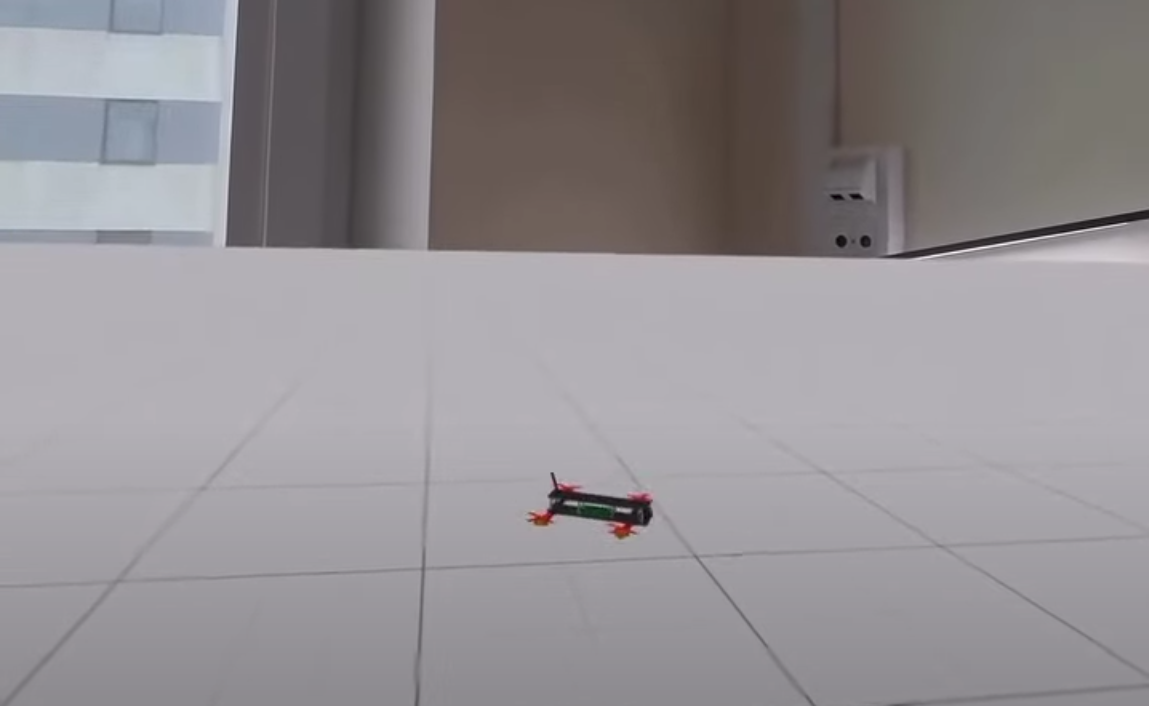
\includegraphics[width=0.8\linewidth]{img/stages/drone-control.png}
\end{figure}